% !TeX spellcheck = en_GB

\documentclass[9pt,journal,compsoc]{IEEEtran}

% The Computer Society requires 12pt.
% If IEEEtran.cls has not been installed into the LaTeX system files,
% manually specify the path to it like:
% \documentclass[10pt,journal,compsoc]{../sty/IEEEtran}

% For Computer Society journals, IEEEtran defaults to the use of 
% Palatino/Palladio as is done in IEEE Computer Society journals.
% To go back to Times Roman, you can use this code:
%\renewcommand{\rmdefault}{ptm}\selectfont





% Some very useful LaTeX packages include:
% (uncomment the ones you want to load)

% Document annotations
%\usepackage[nomargin]{fixme}
%\fxsetup{layout=pdfnote}

% *** MISC UTILITY PACKAGES ***
%
%\usepackage{ifpdf}
% Heiko Oberdiek's ifpdf.sty is very useful if you need conditional
% compilation based on whether the output is pdf or dvi.
% usage:
% \ifpdf
%   % pdf code
% \else
%   % dvi code
% \fi
% The latest version of ifpdf.sty can be obtained from:
% http://www.ctan.org/tex-archive/macros/latex/contrib/oberdiek/
% Also, note that IEEEtran.cls V1.7 and later provides a builtin
% \ifCLASSINFOpdf conditional that works the same way.
% When switching from latex to pdflatex and vice-versa, the compiler may
% have to be run twice to clear warning/error messages.






% *** CITATION PACKAGES ***
%
\ifCLASSOPTIONcompsoc
  % IEEE Computer Society needs nocompress option
  % requires cite.sty v4.0 or later (November 2003)
  \usepackage[nocompress]{cite}
\else
  % normal IEEE
  \usepackage{cite}
\fi
% cite.sty was written by Donald Arseneau
% V1.6 and later of IEEEtran pre-defines the format of the cite.sty package
% \cite{} output to follow that of IEEE. Loading the cite package will
% result in citation numbers being automatically sorted and properly
% "compressed/ranged". e.g., [1], [9], [2], [7], [5], [6] without using
% cite.sty will become [1], [2], [5]--[7], [9] using cite.sty. cite.sty's
% \cite will automatically add leading space, if needed. Use cite.sty's
% noadjust option (cite.sty V3.8 and later) if you want to turn this off
% such as if a citation ever needs to be enclosed in parenthesis.
% cite.sty is already installed on most LaTeX systems. Be sure and use
% version 4.0 (2003-05-27) and later if using hyperref.sty. cite.sty does
% not currently provide for hyperlinked citations.
% The latest version can be obtained at:
% http://www.ctan.org/tex-archive/macros/latex/contrib/cite/
% The documentation is contained in the cite.sty file itself.
%
% Note that some packages require special options to format as the Computer
% Society requires. In particular, Computer Society  papers do not use
% compressed citation ranges as is done in typical IEEE papers
% (e.g., [1]-[4]). Instead, they list every citation separately in order
% (e.g., [1], [2], [3], [4]). To get the latter we need to load the cite
% package with the nocompress option which is supported by cite.sty v4.0
% and later.
%
% Note also the use of a CLASSOPTION conditional provided by 
% IEEEtran.cls V1.7 and later.





% *** GRAPHICS RELATED PACKAGES ***
%
\usepackage[pdftex]{graphicx}
% declare the path(s) where your graphic files are
\graphicspath{{../pdf/}{../jpeg/}}
% and their extensions so you won't have to specify these with
% every instance of \includegraphics
\DeclareGraphicsExtensions{.pdf,.jpeg,.png}



% *** MATH PACKAGES ***
%
\usepackage[cmex10]{amsmath}
\DeclareMathOperator{\prng}{prng}
\DeclareMathOperator{\len}{len}
\DeclareMathOperator{\xorSplit}{xorSplit}
\DeclareMathOperator{\xorMerge}{xorMerge}
\DeclareMathOperator{\splitPayload}{splitPayload}
\DeclareMathOperator{\mergePayload}{mergePayload}
\DeclareMathOperator{\startsWith}{startsWith}
\DeclareMathOperator{\lendsWith}{endsWith}
\DeclareMathOperator{\addRedundancy}{addRedundancy}
\DeclareMathOperator{\removeRedundancy}{removeRedundancy}
\DeclareMathOperator{\encrypt}{encrypt}
\DeclareMathOperator{\decrypt}{decrypt}
% A popular package from the American Mathematical Society that provides
% many useful and powerful commands for dealing with mathematics. If using
% it, be sure to load this package with the cmex10 option to ensure that
% only type 1 fonts will utilized at all point sizes. Without this option,
% it is possible that some math symbols, particularly those within
% footnotes, will be rendered in bitmap form which will result in a
% document that can not be IEEE Xplore compliant!
%
% Also, note that the amsmath package sets \interdisplaylinepenalty to 10000
% thus preventing page breaks from occurring within multiline equations. Use:
%\interdisplaylinepenalty=2500
% after loading amsmath to restore such page breaks as IEEEtran.cls normally
% does. amsmath.sty is already installed on most LaTeX systems. The latest
% version and documentation can be obtained at:
% http://www.ctan.org/tex-archive/macros/latex/required/amslatex/math/





% *** SPECIALIZED LIST PACKAGES ***
%\usepackage{acronym}
% acronym.sty was written by Tobias Oetiker. This package provides tools for
% managing documents with large numbers of acronyms. (You don't *have* to
% use this package - unless you have a lot of acronyms, you may feel that
% such package management of them is bit of an overkill.)
% Do note that the acronym environment (which lists acronyms) will have a
% problem when used under IEEEtran.cls because acronym.sty relies on the
% description list environment - which IEEEtran.cls has customized for
% producing IEEE style lists. A workaround is to declared the longest
% label width via the IEEEtran.cls \IEEEiedlistdecl global control:
%
% \renewcommand{\IEEEiedlistdecl}{\IEEEsetlabelwidth{SONET}}
% \begin{acronym}
%
% \end{acronym}
% \renewcommand{\IEEEiedlistdecl}{\relax}% remember to reset \IEEEiedlistdecl
%
% instead of using the acronym environment's optional argument.
% The latest version and documentation can be obtained at:
% http://www.ctan.org/tex-archive/macros/latex/contrib/acronym/


%\usepackage{algorithmic}
% algorithmic.sty was written by Peter Williams and Rogerio Brito.
% This package provides an algorithmic environment fo describing algorithms.
% You can use the algorithmic environment in-text or within a figure
% environment to provide for a floating algorithm. Do NOT use the algorithm
% floating environment provided by algorithm.sty (by the same authors) or
% algorithm2e.sty (by Christophe Fiorio) as IEEE does not use dedicated
% algorithm float types and packages that provide these will not provide
% correct IEEE style captions. The latest version and documentation of
% algorithmic.sty can be obtained at:
% http://www.ctan.org/tex-archive/macros/latex/contrib/algorithms/
% There is also a support site at:
% http://algorithms.berlios.de/index.html
% Also of interest may be the (relatively newer and more customizable)
% algorithmicx.sty package by Szasz Janos:
% http://www.ctan.org/tex-archive/macros/latex/contrib/algorithmicx/




% *** ALIGNMENT PACKAGES ***
%
%\usepackage{array}
% Frank Mittelbach's and David Carlisle's array.sty patches and improves
% the standard LaTeX2e array and tabular environments to provide better
% appearance and additional user controls. As the default LaTeX2e table
% generation code is lacking to the point of almost being broken with
% respect to the quality of the end results, all users are strongly
% advised to use an enhanced (at the very least that provided by array.sty)
% set of table tools. array.sty is already installed on most systems. The
% latest version and documentation can be obtained at:
% http://www.ctan.org/tex-archive/macros/latex/required/tools/


%\usepackage{mdwmath}
%\usepackage{mdwtab}
% Also highly recommended is Mark Wooding's extremely powerful MDW tools,
% especially mdwmath.sty and mdwtab.sty which are used to format equations
% and tables, respectively. The MDWtools set is already installed on most
% LaTeX systems. The lastest version and documentation is available at:
% http://www.ctan.org/tex-archive/macros/latex/contrib/mdwtools/


% IEEEtran contains the IEEEeqnarray family of commands that can be used to
% generate multiline equations as well as matrices, tables, etc., of high
% quality.


%\usepackage{eqparbox}
% Also of notable interest is Scott Pakin's eqparbox package for creating
% (automatically sized) equal width boxes - aka "natural width parboxes".
% Available at:
% http://www.ctan.org/tex-archive/macros/latex/contrib/eqparbox/




% *** SUBFIGURE PACKAGES ***
%\ifCLASSOPTIONcompsoc
%  \usepackage[caption=false,font=normalsize,labelfont=sf,textfont=sf]{subfig}
%\else
%  \usepackage[caption=false,font=footnotesize]{subfig}
%\fi
% subfig.sty, written by Steven Douglas Cochran, is the modern replacement
% for subfigure.sty, the latter of which is no longer maintained and is
% incompatible with some LaTeX packages including fixltx2e. However,
% subfig.sty requires and automatically loads Axel Sommerfeldt's caption.sty
% which will override IEEEtran.cls' handling of captions and this will result
% in non-IEEE style figure/table captions. To prevent this problem, be sure
% and invoke subfig.sty's "caption=false" package option (available since
% subfig.sty version 1.3, 2005/06/28) as this is will preserve IEEEtran.cls
% handling of captions.
% Note that the Computer Society format requires a larger sans serif font
% than the serif footnote size font used in traditional IEEE formatting
% and thus the need to invoke different subfig.sty package options depending
% on whether compsoc mode has been enabled.
%
% The latest version and documentation of subfig.sty can be obtained at:
% http://www.ctan.org/tex-archive/macros/latex/contrib/subfig/




% *** FLOAT PACKAGES ***
%
%\usepackage{fixltx2e}
% fixltx2e, the successor to the earlier fix2col.sty, was written by
% Frank Mittelbach and David Carlisle. This package corrects a few problems
% in the LaTeX2e kernel, the most notable of which is that in current
% LaTeX2e releases, the ordering of single and double column floats is not
% guaranteed to be preserved. Thus, an unpatched LaTeX2e can allow a
% single column figure to be placed prior to an earlier double column
% figure. The latest version and documentation can be  at:
% http://www.ctan.org/tex-archive/macros/latex/base/


%\usepackage{stfloats}
% stfloats.sty was written by Sigitas Tolusis. This package gives LaTeX2e
% the ability to do double column floats at the bottom of the page as well
% as the top. (e.g., "\begin{figure*}[!b]" is not normally possible in
% LaTeX2e). It also provides a command:
%\fnbelowfloat
% to enable the placement of footnotes below bottom floats (the standard
% LaTeX2e kernel puts them above bottom floats). This is an invasive package
% which rewrites many portions of the LaTeX2e float routines. It may not work
% with other packages that modify the LaTeX2e float routines. The latest
% version and documentation can be obtained at:
% http://www.ctan.org/tex-archive/macros/latex/contrib/sttools/
% Do not use the stfloats baselinefloat ability as IEEE does not allow
% \baselineskip to stretch. Authors submitting work to the IEEE should note
% that IEEE rarely uses double column equations and that authors should try
% to avoid such use. Do not be tempted to use the cuted.sty or midfloat.sty
% packages (also by Sigitas Tolusis) as IEEE does not format its papers in
% such ways.
% Do not attempt to use stfloats with fixltx2e as they are incompatible.
% Instead, use Morten Hogholm'a dblfloatfix which combines the features
% of both fixltx2e and stfloats:
%
\usepackage{dblfloatfix}
% The latest version can be found at:
% http://www.ctan.org/tex-archive/macros/latex/contrib/dblfloatfix/


%\ifCLASSOPTIONcaptionsoff
%  \usepackage[nomarkers]{endfloat}
% \let\MYoriglatexcaption\caption
% \renewcommand{\caption}[2][\relax]{\MYoriglatexcaption[#2]{#2}}
%\fi
% endfloat.sty was written by James Darrell McCauley, Jeff Goldberg and 
% Axel Sommerfeldt. This package may be useful when used in conjunction with 
% IEEEtran.cls'  captionsoff option. Some IEEE journals/societies require that
% submissions have lists of figures/tables at the end of the paper and that
% figures/tables without any captions are placed on a page by themselves at
% the end of the document. If needed, the draftcls IEEEtran class option or
% \CLASSINPUTbaselinestretch interface can be used to increase the line
% spacing as well. Be sure and use the nomarkers option of endfloat to
% prevent endfloat from "marking" where the figures would have been placed
% in the text. The two hack lines of code above are a slight modification of
% that suggested by in the endfloat docs (section 8.4.1) to ensure that
% the full captions always appear in the list of figures/tables - even if
% the user used the short optional argument of \caption[]{}.
% IEEE papers do not typically make use of \caption[]'s optional argument,
% so this should not be an issue. A similar trick can be used to disable
% captions of packages such as subfig.sty that lack options to turn off
% the subcaptions:
% For subfig.sty:
% \let\MYorigsubfloat\subfloat
% \renewcommand{\subfloat}[2][\relax]{\MYorigsubfloat[]{#2}}
% However, the above trick will not work if both optional arguments of
% the \subfloat command are used. Furthermore, there needs to be a
% description of each subfigure *somewhere* and endfloat does not add
% subfigure captions to its list of figures. Thus, the best approach is to
% avoid the use of subfigure captions (many IEEE journals avoid them anyway)
% and instead reference/explain all the subfigures within the main caption.
% The latest version of endfloat.sty and its documentation can obtained at:
% http://www.ctan.org/tex-archive/macros/latex/contrib/endfloat/
%
% The IEEEtran \ifCLASSOPTIONcaptionsoff conditional can also be used
% later in the document, say, to conditionally put the References on a 
% page by themselves.





% *** PDF, URL AND HYPERLINK PACKAGES ***
%
\usepackage{url}
% url.sty was written by Donald Arseneau. It provides better support for
% handling and breaking URLs. url.sty is already installed on most LaTeX
% systems. The latest version and documentation can be obtained at:
% http://www.ctan.org/tex-archive/macros/latex/contrib/url/
% Basically, \url{my_url_here}.


% NOTE: PDF thumbnail features are not required in IEEE papers
%       and their use requires extra complexity and work.
\ifCLASSINFOpdf
  \usepackage[pdftex]{thumbpdf}
\else
  \usepackage[dvips]{thumbpdf}
\fi
% thumbpdf.sty and its companion Perl utility were written by Heiko Oberdiek.
% It allows the user a way to produce PDF documents that contain fancy
% thumbnail images of each of the pages (which tools like acrobat reader can
% utilize). This is possible even when using dvi->ps->pdf workflow if the
% correct thumbpdf driver options are used. thumbpdf.sty incorporates the
% file containing the PDF thumbnail information (filename.tpm is used with
% dvips, filename.tpt is used with pdftex, where filename is the base name of
% your tex document) into the final ps or pdf output document. An external
% utility, the thumbpdf *Perl script* is needed to make these .tpm or .tpt
% thumbnail files from a .ps or .pdf version of the document (which obviously
% does not yet contain pdf thumbnails). Thus, one does a:
% 
% thumbpdf filename.pdf 
%
% to make a filename.tpt, and:
%
% thumbpdf --mode dvips filename.ps
%
% to make a filename.tpm which will then be loaded into the document by
% thumbpdf.sty the NEXT time the document is compiled (by pdflatex or
% latex->dvips->ps2pdf). Users must be careful to regenerate the .tpt and/or
% .tpm files if the main document changes and then to recompile the
% document to incorporate the revised thumbnails to ensure that thumbnails
% match the actual pages. It is easy to forget to do this!
% 
% Unix systems come with a Perl interpreter. However, MS Windows users
% will usually have to install a Perl interpreter so that the thumbpdf
% script can be run. The Ghostscript PS/PDF interpreter is also required.
% See the thumbpdf docs for details. The latest version and documentation
% can be obtained at.
% http://www.ctan.org/tex-archive/support/thumbpdf/

% NOTE: PDF hyperlink and bookmark features are not required in IEEE
%       papers and their use requires extra complexity and work.
% *** IF USING HYPERREF BE SURE AND CHANGE THE EXAMPLE PDF ***
% *** TITLE/SUBJECT/AUTHOR/KEYWORDS INFO BELOW!!           ***
\ifCLASSOPTIONpeerreview
\newcommand\MYhyperrefoptions{bookmarks=true,bookmarksnumbered=true,
	pdfpagemode={UseOutlines},plainpages=false,pdfpagelabels=true,
	colorlinks=true,linkcolor={black},citecolor={black},urlcolor={black},
	pdftitle={Requrirements to send unobservable messages accross the internet},%<!CHANGE!
	pdfsubject={Unobservable Messages},%<!CHANGE!
	pdfkeywords={messages, unobservable}}%<^!CHANGE!
\else
\newcommand\MYhyperrefoptions{bookmarks=true,bookmarksnumbered=true,
pdfpagemode={UseOutlines},plainpages=false,pdfpagelabels=true,
colorlinks=true,linkcolor={black},citecolor={black},urlcolor={black},
pdftitle={Requrirements to send unobservable messages accross the internet},%<!CHANGE!
pdfsubject={Unobservable Messages},%<!CHANGE!
pdfauthor={Martin Gwerder},%<!CHANGE!
pdfkeywords={messages, unobservable}}%<^!CHANGE!
\fi
\ifCLASSINFOpdf
\usepackage[\MYhyperrefoptions,pdftex]{hyperref}
\else
\usepackage[\MYhyperrefoptions,breaklinks=true,dvips]{hyperref}
\usepackage{breakurl}
\fi
% One significant drawback of using hyperref under DVI output is that the
% LaTeX compiler cannot break URLs across lines or pages as can be done
% under pdfLaTeX's PDF output via the hyperref pdftex driver. This is
% probably the single most important capability distinction between the
% DVI and PDF output. Perhaps surprisingly, all the other PDF features
% (PDF bookmarks, thumbnails, etc.) can be preserved in
% .tex->.dvi->.ps->.pdf workflow if the respective packages/scripts are
% loaded/invoked with the correct driver options (dvips, etc.). 
% As most IEEE papers use URLs sparingly (mainly in the references), this
% may not be as big an issue as with other publications.
%
% That said, Vilar Camara Neto created his breakurl.sty package which
% permits hyperref to easily break URLs even in dvi mode.
% Note that breakurl, unlike most other packages, must be loaded
% AFTER hyperref. The latest version of breakurl and its documentation can
% be obtained at:
% http://www.ctan.org/tex-archive/macros/latex/contrib/breakurl/
% breakurl.sty is not for use under pdflatex pdf mode.
%
% The advanced features offer by hyperref.sty are not required for IEEE
% submission, so users should weigh these features against the added
% complexity of use.
% The package options above demonstrate how to enable PDF bookmarks
% (a type of table of contents viewable in Acrobat Reader) as well as
% PDF document information (title, subject, author and keywords) that is
% viewable in Acrobat reader's Document_Properties menu. PDF document
% information is also used extensively to automate the cataloging of PDF
% documents. The above set of options ensures that hyperlinks will not be
% colored in the text and thus will not be visible in the printed page,
% but will be active on "mouse over". USING COLORS OR OTHER HIGHLIGHTING
% OF HYPERLINKS CAN RESULT IN DOCUMENT REJECTION BY THE IEEE, especially if
% these appear on the "printed" page. IF IN DOUBT, ASK THE RELEVANT
% SUBMISSION EDITOR. You may need to add the option hypertexnames=false if
% you used duplicate equation numbers, etc., but this should not be needed
% in normal IEEE work.
% The latest version of hyperref and its documentation can be obtained at:
% http://www.ctan.org/tex-archive/macros/latex/contrib/hyperref/

% *** Do not adjust lengths that control margins, column widths, etc. ***
% *** Do not use packages that alter fonts (such as pslatex).         ***
% There should be no need to do such things with IEEEtran.cls V1.6 and later.
% (Unless specifically asked to do so by the journal or conference you plan
% to submit to, of course. )


% correct bad hyphenation here
\hyphenation{op-tical net-works semi-conduc-tor}

\usepackage{zref-user}
%\usepackage{extsizes}
\usepackage[margin=0.6in]{geometry}
\begin{document}
%
% paper title
% can use linebreaks \\ within to get better formatting as desired
% Do not put math or special symbols in the title.
\title{Sending unobservable messages across the internet}
%
%
% author names and IEEE memberships
% note positions of commas and nonbreaking spaces ( ~ ) LaTeX will not break
% a structure at a ~ so this keeps an author's name from being broken across
% two lines.
% use \thanks{} to gain access to the first footnote area
% a separate \thanks must be used for each paragraph as LaTeX2e's \thanks
% was not built to handle multiple paragraphs
%
%
%\IEEEcompsocitemizethanks is a special \thanks that produces the bulleted
% lists the Computer Society journals use for "first footnote" author
% affiliations. Use \IEEEcompsocthanksitem which works much like \item
% for each affiliation group. When not in compsoc mode,
% \IEEEcompsocitemizethanks becomes like \thanks and
% \IEEEcompsocthanksitem becomes a line break with idention. This
% facilitates dual compilation, although admittedly the differences in the
% desired content of \author between the different types of papers makes a
% one-size-fits-all approach a daunting prospect. For instance, compsoc 
% journal papers have the author affiliations above the "Manuscript
% received ..."  text while in non-compsoc journals this is reversed. Sigh.

\ifCLASSOPTIONpeerreview
\author{}
\else
\author{Martin Gwerder% <-this % stops a space
%\IEEEcompsocitemizethanks{\IEEEcompsocthanksitem none?.\protect\\
% note need leading \protect in front of \\ to get a newline within \thanks as
% \\ is fragile and will error, could use \hfil\break instead.
%E-mail: m.gwerder@unibas.ch
%\IEEEcompsocthanksitem J. Doe and J. Doe are with Anonymous University.}% <-this % stops a space
%\thanks{Manuscript received April 19, 2005; revised December 27, 2012.}
}
\fi

% note the % following the last \IEEEmembership and also \thanks - 
% these prevent an unwanted space from occurring between the last author name
% and the end of the author line. i.e., if you had this:
% 
% \author{....lastname \thanks{...} \thanks{...} }
%                     ^------------^------------^----Do not want these spaces!
%
% a space would be appended to the last name and could cause every name on that
% line to be shifted left slightly. This is one of those "LaTeX things". For
% instance, "\textbf{A} \textbf{B}" will typeset as "A B" not "AB". To get
% "AB" then you have to do: "\textbf{A}\textbf{B}"
% \thanks is no different in this regard, so shield the last } of each \thanks
% that ends a line with a % and do not let a space in before the next \thanks.
% Spaces after \IEEEmembership other than the last one are OK (and needed) as
% you are supposed to have spaces between the names. For what it is worth,
% this is a minor point as most people would not even notice if the said evil
% space somehow managed to creep in.

% The paper headers
\ifCLASSOPTIONpeerreview
\markboth{}{Short Introducton to the MessageVortex Protocol}
\else
%journal: Security \& Privacy,~Vol.~??, No.??, Mai~2015
\markboth{}%
{Gwerder: Short Introducton to the MessageVortex Protocol}
\fi
% The only time the second header will appear is for the odd numbered pages
% after the title page when using the twoside option.
% 
% *** Note that you probably will NOT want to include the author's ***
% *** name in the headers of peer review papers.                   ***
% You can use \ifCLASSOPTIONpeerreview for conditional compilation here if
% you desire.



% The publisher's ID mark at the bottom of the page is less important with
% Computer Society journal papers as those publications place the marks
% outside of the main text columns and, therefore, unlike regular IEEE
% journals, the available text space is not reduced by their presence.
% If you want to put a publisher's ID mark on the page you can do it like
% this:
%\IEEEpubid{0000--0000/00\$00.00~\copyright~2012 IEEE}
% or like this to get the Computer Society new two part style.
%\IEEEpubid{\makebox[\columnwidth]{\hfill 0000--0000/00/\$00.00~\copyright~2012 IEEE}%
%\hspace{\columnsep}\makebox[\columnwidth]{Published by the IEEE Computer Society\hfill}}
% Remember, if you use this you must call \IEEEpubidadjcol in the second
% column for its text to clear the IEEEpubid mark (Computer Society journal
% papers don't need this extra clearance.)



% use for special paper notices
%\IEEEspecialpapernotice{(Invited Paper)}

% for Computer Society papers, we must declare the abstract and index terms
% PRIOR to the title within the \IEEEtitleabstractindextext IEEEtran
% command as these need to go into the title area created by \maketitle.
% As a general rule, do not put math, special symbols or citations
% in the abstract or keywords.
\IEEEtitleabstractindextext{%
\begin{abstract}
In this paper we introduce an unobservable message annonymisation protocol, named MessageVortex. It is based on the zero trust principle and a distributed peer-to-peer (P2P) architecture and avoids  central aspects such as fixed infrastructures within a global network. It scores over existing work by blending its traffic into suitable existing transport protocols, thus making it next to impossible to block it without significantly affecting regular users of the transport medium. It furthermore requires no protocol-specific infrastructure in public networks and allows a sender to control all aspects of a message such as degree of anonymity, timing, and redundancy of the message transport without disclosing any of these details to the routing or transporting nodes.
\end{abstract}

% Note that keywords are not normally used for peerreview papers.
\begin{IEEEkeywords}
Data privacy, Message systems, Anonymity, Security
\end{IEEEkeywords}}


% make the title area
\maketitle


% To allow for easy dual compilation without having to reenter the
% abstract/keywords data, the \IEEEtitleabstractindextext text will
% not be used in maketitle, but will appear (i.e., to be "transported")
% here as \IEEEdisplaynontitleabstractindextext when compsoc mode
% is not selected <OR> if conference mode is selected - because compsoc
% conference papers position the abstract like regular (non-compsoc)
% papers do!
\IEEEdisplaynontitleabstractindextext
% \IEEEdisplaynontitleabstractindextext has no effect when using
% compsoc under a non-conference mode.


% For peer review papers, you can put extra information on the cover
% page as needed:
% \ifCLASSOPTIONpeerreview
% \begin{center} \bfseries EDICS Category: 3-BBND \end{center}
% \fi
%
% For peerreview papers, this IEEEtran command inserts a page break and
% creates the second title. It will be ignored for other modes.
\IEEEpeerreviewmaketitle



\section{Introduction}
% Computer Society journal papers do something a tad strange with the very
% first section heading (almost always called "Introduction"). They place it
% ABOVE the main text! IEEEtran.cls currently does not do this for you.
% However, You can achieve this effect by making LaTeX jump through some
% hoops via something like:
%
%\ifCLASSOPTIONcompsoc
%  \noindent\raisebox{2\baselineskip}[0pt][0pt]%
%  {\parbox{\columnwidth}{\section{Introduction}\label{sec:introduction}%
%  \global\everypar=\everypar}}%
%  \vspace{-1\baselineskip}\vspace{-\parskip}\par
%\else
%  \section{Introduction}\label{sec:introduction}\par
%\fi
%
% Admittedly, this is a hack and may well be fragile, but seems to do the
% trick for me. Note the need to keep any \label that may be used right
% after \section in the above as the hack puts \section within a raised box.



% The very first letter is a 2 line initial drop letter followed
% by the rest of the first word in caps (small caps for compsoc).
% 
% form to use if the first word consists of a single letter:
% \IEEEPARstart{A}{demo} file is ....
% 
% form to use if you need the single drop letter followed by
% normal text (unknown if ever used by IEEE):
% \IEEEPARstart{A}{}demo file is ....
% 
% Some journals put the first two words in caps:
% \IEEEPARstart{T}{his demo} file is ....
% 
% Here we have the typical use of a "T" for an initial drop letter
% and "HIS" in caps to complete the first word.
\IEEEPARstart{S}{ince} whistle blower Edward Snowden disclosed documents, it seems generally accepted that global monitoring of Internet traffic is conducted. According to these documents (verified by \href{http://www.nrc.nl/nieuws/2013/11/23/nederland-sinds-1946-doelwit-van-nsa}{NRC}) NSA infiltrated more than 50k computers with malware to collect classified or personal information. They furthermore infiltrated telecom operators such as Belgacom to collect data, and targeted high members of governments even in associated states. 

A message sent throughout the Internet must, even when perfectly encrypted, disclose at least the recipient to the router transporting a message. The sender can be identified by the return path or is identifiable by following the source of packets. Meta information is valuable, because frequency and message size disclose important facts about the association and intensity of the relationship of involved parties. %Typical attacks are traffic capturing by network observation or by inserting one or more malicious nodes into a routing network. 

This paper addresses the above-mentioned problems of traffic monitoring by introducing a new  protocol called MessageVortex. Within MessageVortex we consider the whole network as untrusted with the exception of the sending and receiving node. MessageVortex does not leak routing information as only the immediate peers are known to a node. The protocol is able to sustain anonymity\cite{anon_terminology} even under harsh assumptions such as an adversary possessing a huge but limited funding, unlimited monitoring capability on the network and a considerable number of own nodes. For a more precise adversary model, see appendix~\ref{sec:adversary}.

Numerous attempts such as in \cite{minion-design,babel,mixmaster-spec,tor-design,freehaven-berk,herbivore:tr} have been made to anonymise message flow. But most of them have problems as they rely at least on the partial trust in the nodes routing the messages, or some central infrastructures \cite{hs-attack06,esorics13-cellflood,esorics12-torscan,oakland2013-trawling}. Exit and entry points are important as they may leak information which is otherwise well hidden within the network. By degrading the network, message flows can be redirected and information extracted from the new flows. Additionally, a dedicated transport protocol is easy to block since their implementation can be easily identified by used ports or some protocol properties. Furthermore, most approaches require infrastructure with fixed addressing in the internet, rendering owners vulnerable.

All papers analysed for this work introduced a new transport layer solving these problems. Only TOR defined an additional transporting mechanism which may be used as an alternate transport medium between two defined nodes to avoid detection. In our approach we decouple the routing layer from the transport layer completely. By doing so we introduce new degrees of complexity to attack scenarios, as messages may use any common transport protocol of the used network. 

Our work consists of a routing layer which is completely P2P based without any central protocol specific infrastructure. Any node is a routing node and may be an endpoint. There is no implicit or explicit trust in any particular system of the  network. Decoy traffic generation is controlled by the original sender of a message. Even a decoy traffic generating node is unable to differentiate between message and decoy traffic as a Solomon-Reed algorithm is used to blow the message up by adding redundancy information. This redundancy information may be decoy traffic or later required to rebuild data blocks. The redundant blocks are always encrypted and a multitude of the cyphers block size as they are padded before splitting. This eliminates the need of padded encryption at block level. This fact makes it very hard to apply brute force in order to decrypt the content. This is due to the fact  that padding no longer hints gives whether decryption has been successful or not.

As transport media we use common, well known store-and-forward-based protocols. By doing so the routing logic has no affiliation to the transport layer. Literally any free-mailer email address or chat account may be converted into a transport media for our protocol without any modification required on the server side. This makes the network very agile on one side at the cost of reliability, as nodes may suddenly appear or disappear. To counter this phenomenon, we are able to introduce a high degree of redundancy if required and wished by the routing block builder.

Using the MessageVortex protocol, any device with a latent or permanent connectivity to the Internet may act as routing node. 

By applying the zero trust model we give full control of all traffic to the original sender of the message. He controls message flow, redundancy, degree of anonymity, timing, and many more aspects of the message transport throughout the whole network. This is done without disclosing any of these parameters to the participating nodes as they are encoded in the operations and only visible to the node executing them. The operations itself are chosen in such a way that they do not reveal the nature of the traffic.

To limit possibilities of denial-of-service (DoS) within the system and guarantee an efficient handling of messages, MessageVortex nodes (in short ``node'') rely on unlinked, ephemeral identities which are created in a proof of work system (PoW). While it is technically easy to use a node, it is hard to carry out traditional attacks against them as all transactions have to be pre-authenticated with PoW puzzles. The amount of work required to disrupt services or conduct traditional attacks against the system grows significantly due to the non linear growth of calculation power required when maintaining more ephemeral identities. It is, however, still possible to exhaust external resources such as network bandwidth.\par\nopagebreak
%\ifCLASSOPTIONpeerreview
%\else
%\hfill gwm\par\nopagebreak
%\hfill Mai 27, 2015
%\fi
\subsection{Previous Work}
Generally not many technologies are usable to achieve anonymity or unlinkability as defined in \cite{anon_terminology}. Most analysed protocols use relays\cite{CHAUM1}, mixes\cite{CHAUM1}, or Dining-Cryptographers-related-networks\cite{chaum-dc} or their variants to achieve anonymisation. Numerous protocols have evolved from these technologies:
\begin{itemize}
	\item \emph{TOR}\cite{tor-design}: Mixer-based infrastructure for tunnelling TCP-based protocol streams. TOR is a synchronous or near synchronous routing system. The anonymisation is based on mixing by using a statical path consisting of an entry node, an exit node and at least three more intermediate nodes.
	\item \emph{mixmaster}\cite{mixmaster-spec}: A type-II remailer where all mixes may choose the path on their own logic.
	\item \emph{Babel}\cite{babel}: Mixer-based remailer where the sender chooses the path and sends an onionised message.
	\item \emph{Mixminion}\cite{minion-design}: A type-III remailer offering sender anonymity. Unlike their predecessors, it is no longer based on the SMTP transport protocol. This system requires at least a centralised directory infrastructure.
	\item \emph{Freehaven}\cite{freehaven-berk}: A distributed storage system. The system offers anonymous document storage. To receive a document, a hash of a public key used to sign the document must be known. Known documents may be identified and owners of infrastructure might be held responsible if hosting such well known, forbidden documents.
	\item \emph{Freenet}\cite{freenet}: Freenet is an anonymous, distributed data storage system. The system does not trust any server. Instead a reputation system is used. This system has attracted very little attention from the researcher community.
	\item \emph{Herbivore}\cite{herbivore:tr}: A DC-net-based protocol without client implementation.
	\item \emph{$\mathcal{P}^5$}\cite{sherwood2005p5}: There is a simulator available for this protocol. Real world implementations do not exist and therefore no attack schemes have been elaborated so far.
	\item \emph{$I^2P$}(\href{https://geti2p.net/}{geti2p.net}): P2P-based pseudonymous protocol allowing TCP and UDP streams to be tunnelled synchronously or near-synchronously. Unlike TOR, $I^2P$ works pseudonymously and mixes using packet switching. 
	%\item \emph{Dissent}\cite{Corrigan-Gibbs:2010:DAA:1866307.1866346}: 
\end{itemize}

Our protocol differs from these works in several ways. There is no central network infrastructure. There are no entry or exit nodes which might be blocked. All nodes including the sender and the recipient are treated equal. The number of nodes, the traffic to be generated, anonymity sets, timing of the message, redundancy in message transmission, and size of all packages to be sent along is solely decided by the builder of a routing block. The builder is normally synonymous to the sender but might be the recipient of a message in case of a reply block. Furthermore, there is no dedicated transport protocol. Instead, MessageVortex messages  (in short ``vmessages'') are embedded in other existing Internet protocols. The traffic itself is mixed by operations. As traffic is generated reproduceable, either by adding redundancy information or by using PRNG with a defined seeding, decoy traffic cannot be differentiated from required blocks.

\section{Methods and Material}

% needed in second column of first page if using \IEEEpubid
%\IEEEpubidadjcol
%\begin{figure}[htb]
%\centering
%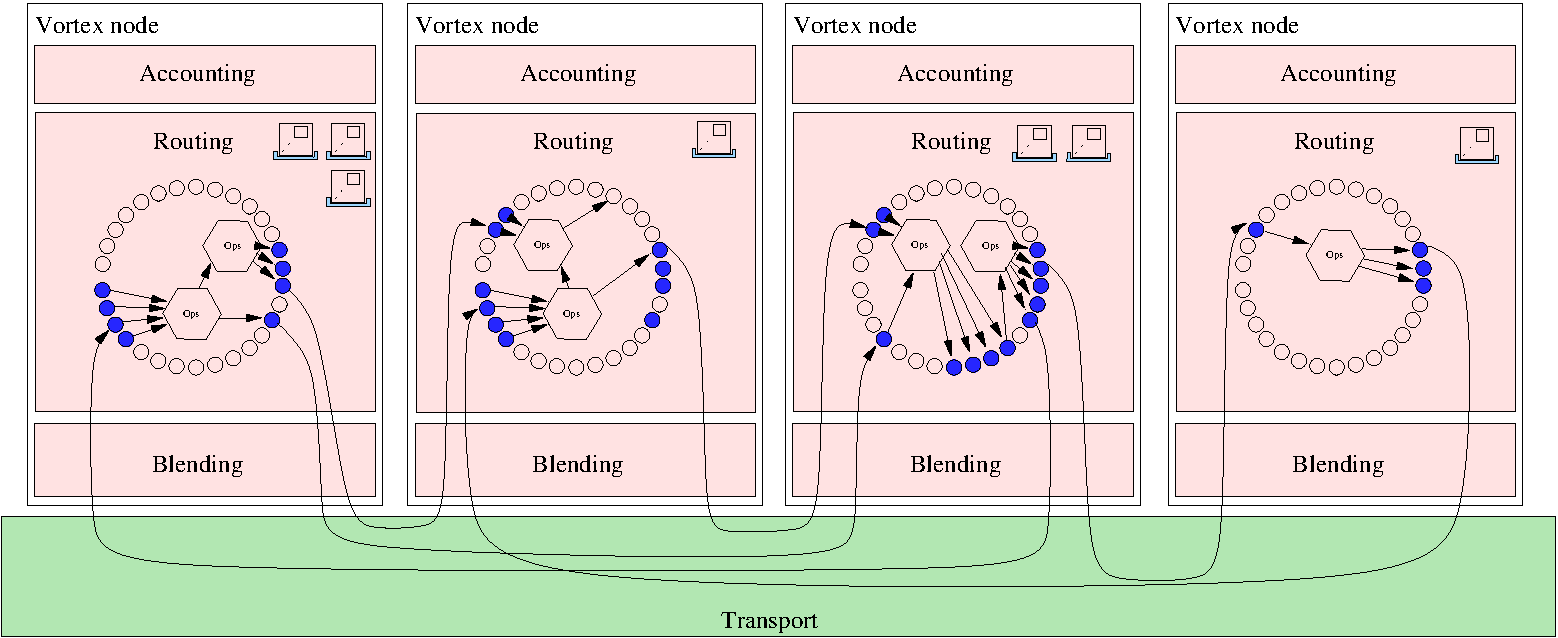
\includegraphics[width=2.5in]{../inc/roughProtocolDesign}
%\caption{Protocol stack.}
%\label{fig:layers}
%\end{figure}
We define the protocol on three different layers:
\begin{itemize}
	\item \emph{Blending layer:} in this layer we embed MessageVortex message into the transport protocol. 
	\item \emph{Routing layer:} this layer applies the logic to the message routing and prepares the message for the blending layer.
	\item \emph{Accounting layer:} this layer is a DoS and misuse protection. It keeps track of the transfers for each ephemeral identity and makes sure that queue and storage capacity are efficiently handled.     
\end{itemize}
These three layers are connected through a fourth existing layer. This layer is based on one or more store-and-forward based, common internet transport protocols. Protocols on this layer we refer in general as transport protocols. It is important to note that no modification is applied to the transport protocol to accommodate vmessages.

All cryptographic operations such as encryption, decryption, hashing, or random number generation do not rely on a single algorithm. The protocol is able to signal what capabilities a node has and how exactly a message should be processed. This makes the protocol very robust if a used algorithm is broken. For this reason, we defined for each capability at least two algorithms which depend on different mathematical puzzles (e.g. ``integer factorisation problem'' versus ``discrete logarithms problem''). This introduces a redundancy in algorithms, allowing a sender to switch between algorithms if required.

\subsection{Protocol Layers}
\subsubsection{Transport}
The transport layer provides the Internet infrastructure. Unlike in most other approaches such as \cite{tor-design,sherwood2005p5,freenet} this layer is not protocol specific. We use already existing, symmetrically built store and forward protocols. Attributes such as anonymity do not rely on the security of this layer.

By using this approach we remove the need for shaky technologies such as TCP or UDP hole punching to connect peer partners. It furthermore makes the use of ``mostly connected'' clients such as mobile phones or DSL connections suitable for this protocol. This is because our transport endpoints are always reachable within the global network. The routing nodes may disconnect from time to time without affecting reachability of an mix. 

Protocols on this layer are typically well known and frequently used. They have no prerequisite for encryption or privacy and are store-and-forward based protocols with routing capabilities. 

\subsubsection{Blending}
This layer is a translation-only layer and embeds vmessages from the routing layer in transport protocol messages. Incoming vmessages are extracted from the transport layer and passed to the routing layer. Messages can be identified by picking a potential vmessage block up and start decyphering $k_{p_N}$ using its private key $k^{-1}_{h_N}$. If decryption succeeds a vmessage block is found. This makes it impossible for an adversary to detect the presence of a vmessage without the hosts private key $k^{-1}_{h_N}$.

Protocol features such as anonymity or redundancy do not rely on this level. This layer embeds messages within the transport layer in such a way that an adversary is no longer able to identify vmessages from regular transport layer messages. Good blending is achieved if transport layer censorship measurements such as application level firewalls are unable to detect the difference between real world messages and vmessages. In an ideal application, this applies to censorship applied by humans as well as censorship applied on the base of algorithms. 

In a real scenario, it is hard to achieve human proof censorship circumvention. If not done with care, problems as described in \cite{abadi2005moderately} arise. It is in our case not necessary as human censorship is very costly and slow compared to algorithms. Human censorship is too slow for real time censorship. Our transport layer is by definition frequently used for regular communication. We always consider an algorithm-based censorship as existing.

Currently, the specification of this layer is limited to the two capabilities ``embed with offset'' and ``F5''. 

``Embed with offset'' is a plain embedding of a block in a file attached to a message. The offset allows issuing first a valid header of some sort in order to improve blending (e.g. for a PCM-encoded WAV file). While this is considered a very weak protection, analysis to detect such a file on a global transport scale is very demanding due to the sheer mass to be analysed. 

``F5'' means applying the F5 algorithm to hide a message within a random suitable jpeg image. ``F5'' is one of the very few steganographic works which have a real world implementation and attracted at least some interest in the research community. In \cite{steganalysisf5}, an approach to detect embedded information in steganographically modified images is presented. To obtain this information, a considerable effort in terms of calculation power is required. This makes it impractical for real time censorship on our scale. It does however allow messages to be identified. Furthermore, It only discloses the fact that F5 is being used. It does not leak the content of a message, its immediate sender (apart from a socket), or a message size.

\subsubsection{Routing}
The routing layer is the mixer of the system. It processes messages extracted by the blending layer and is supported by the accounting layer. Any related set of messages is processed by the routing layer by recombining payload with operations defined in section~\ref{sec:operations}. Due to the nature of these operations, a node is unable to tell whether the traffic flow processed is decoy traffic or an actual part of the message flow.

If a message is processed a new vmessage is generated and passed on to the blending layer.

For a more precise working of the routing process see section~\ref{sec:processing}.

\subsubsection{Accounting}
The accounting layer protects a node from being overloaded or misused. Every sender must first apply for an ephemeral identity which is limited in lifetime. This is done by a proof of work algorithm. When an ephemeral identity is created the owner of the identity may route vmessages through a node. The ephemeral identity is assigned with message and size transfer quotas. Any identity may apply for a raise of quota as long as it is not expired. It is up to the node to decide whether a raise of quota is acceptable or not. If rejected, any sender might try to apply for a new ephemeral identity.

Due to the costs of maintaining multiple identities and their parental identities for anonymity of the original sender, the number of identities grows exponentially when growing a network of ephemeral identities. A sender might either introduce a new node to cut identity costs or maintain at higher identity costs a single node.

\subsection{Protocol Outline}
We define a protocol block which has an inner block structure as shown in Fig~\ref{fig:blocks}.

\begin{figure}[htb]
	\centering
	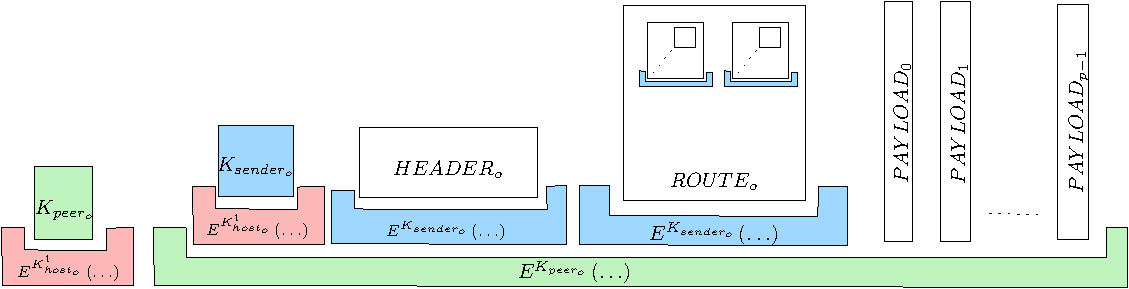
\includegraphics[width=\columnwidth]{../inc/blockLayoutSimplified}
	\caption{Protocol block outline.}
	\label{fig:blocks}
\end{figure}

These blocks are passed from node to node. All blocks are binary proof, which means that the same block sent twice will always result in exactly the same bit layout. There is no room for a misbehaving node to tag the block within it without compromising the message. The message as a whole is replay protected. Routing and header blocks are linked with a chain secret to avoid hijacking of header or routing blocks.

\subsubsection{Message Keys}
Every protocol block is protected by two symmetric keys $key_{peer_N}$ (in short $k_{p_N}$) , $key_{sender_N}$ (in short $k_{s_N}$) and the private part of an asymmetric host key $k^{-1}_{host_N}$ (in short $k^{-1}_{h_N}$). The public host key $k^{1}_{h_N}$ and both symmetric keys are known to the builder of the routing block structure. 

This building is done by the sender. If using SURBs (Single Use Reply Blocks) or MURBs (Multi Use Reply Blocks) it is done by the builder of the reply block. 

The header is protected by the symmetric key $k_{s_N}$ and is found in a preamble to the header protected by the receiving peer's private key $k^{-1}_{h_N}$. The key $k_{s_N}$ is known to the routing block builder and the receiving node only. The receiving node obtains all important information protected by this key. $k_{p_N}$ is known to two immediate peers and the builder of the routing block. The sending peer obtains $k_{p_N}$ from the routing block, whereas the receiving peer acquires it in the $headerBlock$. 

\subsection{Pad Block}
The pad block is a short block of a few bytes of padding content (first bytes of the first message block; fixed size per message; null padded) guaranteeing that all messages sent with the same routing block look different on the transport layer.

\subsubsection{Header Block}
The header block contains vital static information for the message disclosed to only one peer of the network. It is protected by key $k_{s_N}$. The minimally contained information can be described by the list $headerBlock_i:=\langle sendingIdentity,\allowbreak{} serial_i,\allowbreak{} replayAttributes_i,\allowbreak{} key_{p_i},\allowbreak{} chainSecret,\allowbreak{} signature,\allowbreak{} optionalOperations \rangle$.

\subsubsection{Routing Block}
A routing block can be expressed with the following recursive definition $routingBlock_i:=\langle\allowbreak{} nexthopAddress,\allowbreak{} chainSecret,\allowbreak{} timingAttributes,\allowbreak{} E^{k_{s_{i+1}}}\left(headerBlock_{i+1}\right),\allowbreak{} E^{k_{s_{i+1}}}\left(routingBlock_{i+1}\right),\allowbreak{} payloadBuildInstructions_i,\allowbreak{} payloadId,\allowbreak{} optionalReplyBlocks \rangle$

\subsubsection{Payload Block}
A payload block is any number of bytes representing parts of a message, decoy traffic or a control block.

\subsection{Message Processing\label{sec:processing}}
Unlike with a traditional mix system, a node has no choice of sending. It purely relies on the message processing facilities. A message is either handed over to the transport layer by the blending layer or may be induced internally (if the local node is the sender). 

First, the preamble to the header is extracted. This proves that the sender possesses the public key of the node and contains the sender key $k_{s_i}$. With this information, the node opens the $headerBlock$ revealing information regarding the ephemeral identity of the original sender. Based on the information given in the relatively small header, the transport layer may decide whether further processing is desired or not. If desired, the node extracts the key $k_{p_i}$ and decrypts the rest of the message, which is considerably larger containing routing and payload information.

The routing block may contain instructions on processing information contained in this or any message related to this message and identity. These instructions are encoded in so-called ``Operations'' as specified in section~\ref{sec:operations} and may be any combination of them. As soon as the time arises for a routing block to be processed, the operations building the new message blocks are executed. If all prerequisites are satisfied, the new payload blocks are built, concatenated with the new routing block, pad, and header block. This resulting block is encrypted with $k_{p_{i+1}}$ and prepended with the preamble. The built block is passed to the blending layer with the blending specification and the target address.

It is important to note that the blending specification contains vital information about how the message must be blended but not how the carrier message looks like. By doing so we avoid abuse of the blending layer (eg. sending plain text spam through the MessageVortex system).

\subsection{Operations\label{sec:operations}}
The operations are designed in such a way that they allow  variance of message size without telling anyone, including the generator, which message part is used later. They include features to protect message content from bugging.

Some of the operations require a pseudo random number generator (PRNG). This PRNG is defined in appendix~\ref{sec:prng}. The definition of a reproduceable PRNG to be used by messages is important as we have to achieve binary proof messages.

All interactions are non-interactive. Interactive operations such as DC-nets do add more complexity to the system. Behavioural analysis can be used to identify interactive operations. 

This is the reason why DC-nets are not used. Theoretically, it is possible reflect them as a single operation by calculating the answer and then broadcasting the answer. In practice, this fails due to the non-existence of efficient, reliable multicast networks. There are however attempts to apply DC-nets to real protocols \cite{Corrigan-Gibbs:2010:DAA:1866307.1866346}.

\subsubsection{$\addRedundancy$ and $\removeRedundancy$ Operation}
This operation is based on a modified Reed-Solomon redundancy function in order to accommodate the anonymity needs of this function. The Reed-Solomon function as defined in appendix~\ref{sec:reedSolomon} offers a varying number of redundant checksum blocks. When sending these blocks into multiple directions no mixing node is able to tell where the original message is being rebuilt. The general inner workings are described in Fig~\ref{fig:addRedundancy}.

\begin{figure}[htb]
	\centering
	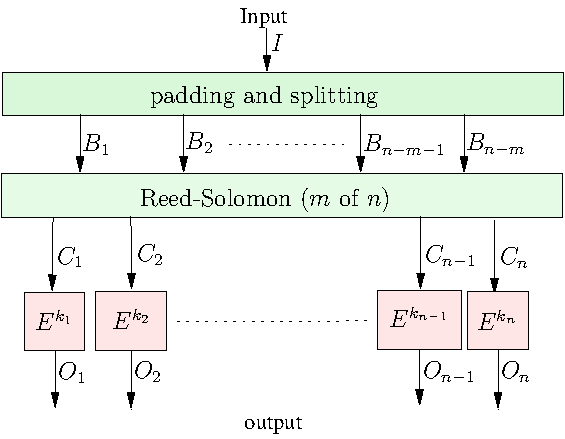
\includegraphics[width=2.5in]{../inc/addRedundancyOp}
	\caption{AddRedundancy Operation}
	\label{fig:addRedundancy}
\end{figure}

We define a function $\addRedundancy_{n,m}( \mathbf{M},k_1\ldots k_{m} )$ where $M$ denotes the message, $n$ the number of total output blocks, $m$ the number of redundancy blocks wheras $m<n$, $k$ the encryption key and scheme to be used, and $bs_k$ the block size required to accommodate scheme and key size described by $k$. It is important to note that the number of true data blocks is $d=n-m$, while the rest of the output blocks are redundant information.

By encrypting all output blocks individually we make sure that no node having access to enough blocks may rebuild the data stream without the routing block builder's consent.

The message is length prefixed with a big endian 64 bit unsigned integer number and padded in such a way that $8+\len(M)+\len(padding) \bmod bs_k =0$. As padding stream, we take the output of $\prng_i\left(\left\lceil\frac{8+\len(M)}{b_s}\right\rceil b_s n\right )$. The first 64 bytes of the message (padded with 0 if required) are taken as initialiser $i$ for the PRNG function. By preparing our message block in such a way, we guarantee that the output blocks are encryptable without further padding and that the output of all $addRedundancy$ functions is binary proof. If stream cyphers are used as output cyphers, then padding is not required.

The reverse function for $\addRedundancy$ is called $\removeRedundancy_{m,n}(B_1\ldots B_{m},k_1\ldots k_{m})=\mathbf{M}$ and recovers the original data stream if enough blocks (at least $m$) and respective valid keys are provided. 

\subsubsection{$\splitPayload$ and $\mergePayload$ Operation}
The $\splitPayload$ and $\mergePayload$ operations split and merge payload blocks ($pb_N$)into two chunks of different or equal sizes respectively joins them. We define the functions as follows:

If $\len(pb_1)$ expresses the size of a payload block called $pb_0$ in bytes then the two resulting blocks of the $splitPayload$ Operation $pb_1$ and $pb_2$ have to follow the following rules:

\begin{eqnarray}
\splitPayload(f, pb_0) & = &\langle pb_1, pb_2 \rangle\\
\startsWith(pb_0, pb_1)\\
\lendsWith(pb_0, pb_2)\\
\len(pb_2) & = & \left\lfloor \len(pb_0)\cdot f\right \rfloor\\
\len(pb_0) & = & \len(pb_1) + \len(pb_2)
\end{eqnarray}
respectively
\begin{eqnarray}
\mergePayload(pb_1, pb_2) & = & pb_0 \\
\startsWith(pb_0, pb_1)\\
\lendsWith(pb_0, pb_2)\\
\len(pb_0) & = & \len(pb_1) + \len(pb_2)
\end{eqnarray}
 
\subsubsection{$\xorSplit$ and $\xorMerge$ Operation}
$\xorSplit$ and $\xorMerge$ are low cost obfuscation operations. These operations may be applied if a block is passed on without any required operation or as one-to-two blocks redundancy generating function. 

The operations are defined as follows:
\begin{eqnarray}
\xorSplit(pb_0) & = &\langle pb_1, \prng_i(\len(pb_0)) \rangle\\
pb_1 & = & pb_0 \oplus \prng_i(\len(pb_0))\\
\xorMerge(pb_1,pb_2) & = &\langle pb_0 \rangle\\
pb_0 & = & pb_1 \oplus pb_2
\end{eqnarray}

\subsubsection{$\encrypt$ and $\decrypt$ Operation}
$\encrypt$ and $\decrypt$ are used as message obfuscation operations. These operations may be applied if a block is passed on without any required operation. They minimise the risk for a known plain text attack to a MessageVortex block. Both operations are defined as a padded or unpadded symmetrical encryption. $spec$ is the encryption specification and key provided by the routing block.

The operations are defined as follows:
\begin{eqnarray}
\encrypt(pb_0) & = & pb_1 \\
\len(pb_1) & \geq & \len(pb_0)\\
\decrypt(pb_1) & = & pb_0
\end{eqnarray}

\subsection{Protocol Bootstrapping}
In order to allow bootstrapping of the protocol, any node may reveal a very small, fixed number of nodes known to it. This allows fresh nodes to bootstrap their knowledge about an existing network, given they know at least one node willing to reveal other nodes. 

Allowing this kind of bootstrapping has certain downsides. As no trust is given into the requester's identity, we have to be very careful here not to reveal the full network to any adversary. By applying the PoW and requiring an ephemeral identity, we assign a high cost to this operation. 

Another downside is that it takes a long time for such a network to balance its loads if a network increases over time in size. Mature nodes concentrate more traffic on them than younger ones. This does however distribute more evenly over time if algorithms as shown in \cite{messageVortex} are applied.

\section{Results}
Our protocol can be seen as tool set for creating and sending anonymised messages. The degree of anonymity and redundancy is created when building the routing block. This is why constraints on message building are important.

\subsection{Message Building}
\begin{figure}[htb]
	\centering
	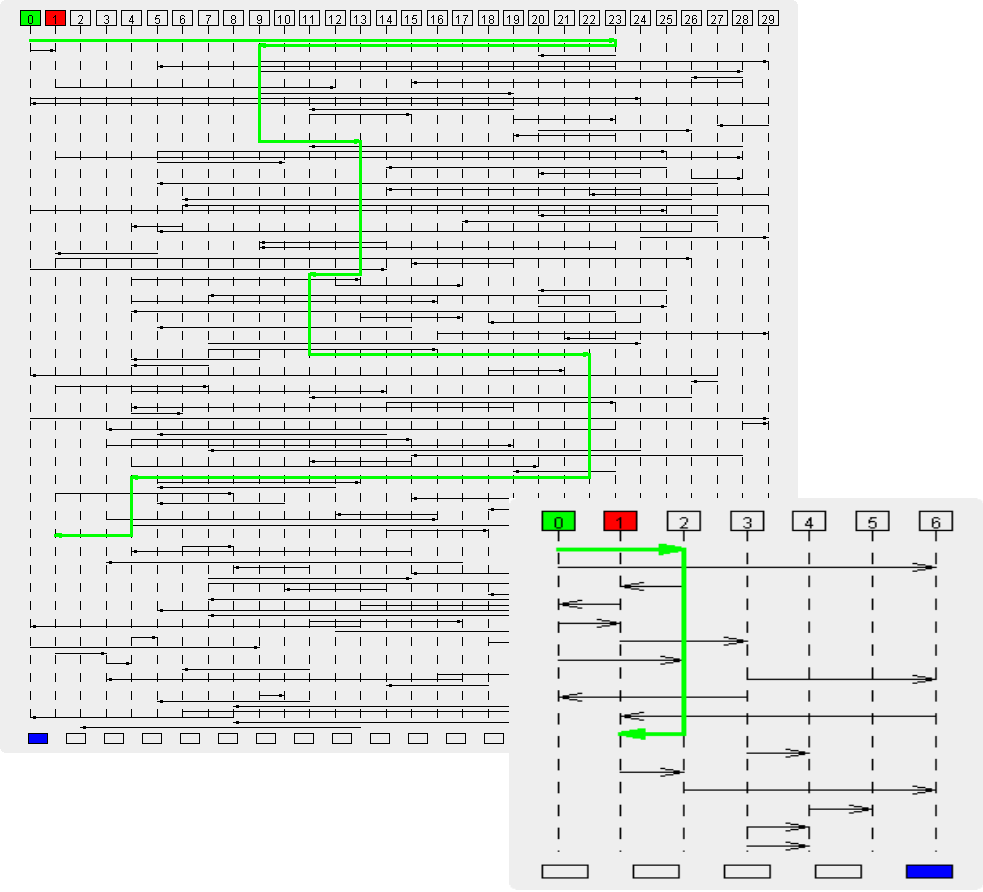
\includegraphics[width=0.8\columnwidth]{msgGraph3}
	\caption{Message graphs with different numbers of nodes}
	\label{fig:mgsGraph}
\end{figure}

Using previously defined operations we may build a message path. This path is typically built by first assigning an identity set $I_k$ where  $k$ denotes the target identity. $I_k$ is a static set of $n$ ephemeral identities $I_k\langle eI_1 \ldots eI_n\rangle$ which are always used to communicate with $k$. This set may be enriched with further $m$ ephemeral identities when sending. An identity set is replaced with a different one as soon as ephemeral identities expire. Therefore, we apply a new anonymity set unrelated to the old one with each new set of ephemeral identities.

A full message graph including all traffic may have any type of complexity. Fig~\ref{fig:mgsGraph} shows a graph with a $k$-Anonymity of $k=7$ of a message. It features 5 partially independent routes from source (edge 0) to the target (edge 1). One is highlighted in green. All involved nodes receive enough information to build the entire message if provided with the correct decoding instruction. X-axis shows involved nodes and y-axis denotes the sequence in time. In its background a graph with $k=30$ and 20 partially independent paths is shown.

When building the message it has to be ensured that all nodes in $I_k$ obtain enough information to rebuild the message. If an adversary is able to identify the full message flow and knows all the operations applied to the message except for those on the entry and exit node and at least a subset of $k=|I_{k_{uncompromised}}|$ where $k>1$ exists then we are still at $k$-Anonymity as an absolute worst case scenario. Thus we can prove that attacks as described in \cite{DanSer04} are of very limited use. 

\subsection{Attacking the Message Flow}
In our thesis\cite{messageVortex} we analyse various kinds of attacks. Such as illicit behaving nodes, hijacking of header and routing blocks, analysis on payload blocks, traffic replay, analysis on infrastructure, and analysis on operations. Results have shown that the protocol is very resistant against most kinds of attacks.

For block hijacking of a single block we can proof that probability for success is at least below $10E-11$. We can furthermore prove the effectiveness of replay protection even when assuming misbehaving nodes. Hijacking a routing block has very limited use however. Prepending an own identity block to a hijacked routing block would break the message path. Thus, allowing an adversary to reveal all blocks built from this routing block out of the message travelling through the adversary node. He does not gain any information about other blocks. He may extract how much traffic is generated on the manipulated node out of these blocks. The real amount of traffic is, however, higher as some operations may have failed due to missing blocks.

We can easily show the effectiveness of the tagging and bugging protection. A misbehaving node has no room to tag a message without compromising the message's integrity. A tagged message will be discarded at the first non-misbehaving node.

\subsection{Routing Diagnosis}
If an interruption of path is suspected, parts of the message may be obtained by the message block builder at any time. He may do this by either introducing fixed diagnostic paths into a routing block, which we refer to as implicit diagnosis, or he may send a second message picking up a block of the message at a node to be tested. This we refer to as explicit diagnostic.

Explicit diagnostics may be used as a kind of ``receipt'' from any node including but not limited to the terminal receiver of a message. Any block at any time of routing may be returned directly or indirectly to the original sender. Arrival of such a packet and content tells the sender at which point a message failed. If a diagnostic packet does not arrive, the routing block builder may build a diagnostic message picking up random packets on any suspected failing node.

% An example of a floating figure using the graphicx package.
% Note that \label must occur AFTER (or within) \caption.
% For figures, \caption should occur after the \includegraphics.
% Note that IEEEtran v1.7 and later has special internal code that
% is designed to preserve the operation of \label within \caption
% even when the captionsoff option is in effect. However, because
% of issues like this, it may be the safest practice to put all your
% \label just after \caption rather than within \caption{}.
%
% Reminder: the "draftcls" or "draftclsnofoot", not "draft", class
% option should be used if it is desired that the figures are to be
% displayed while in draft mode.
%
%\begin{figure}[!t]
%\centering
%\includegraphics[width=2.5in]{myfigure}
% where an .eps filename suffix will be assumed under latex, 
% and a .pdf suffix will be assumed for pdflatex; or what has been declared
% via \DeclareGraphicsExtensions.
%\caption{Simulation Results.}
%\label{fig_sim}
%\end{figure}

% Note that IEEE typically puts floats only at the top, even when this
% results in a large percentage of a column being occupied by floats.
% However, the Computer Society has been known to put floats at the bottom.


% An example of a double column floating figure using two subfigures.
% (The subfig.sty package must be loaded for this to work.)
% The subfigure \label commands are set within each subfloat command,
% and the \label for the overall figure must come after \caption.
% \hfil is used as a separator to get equal spacing.
% Watch out that the combined width of all the subfigures on a 
% line do not exceed the text width or a line break will occur.
%
%\begin{figure*}[!t]
%\centering
%\subfloat[Case I]{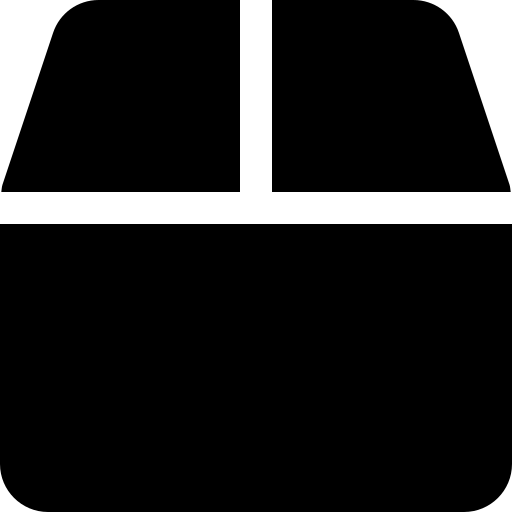
\includegraphics[width=2.5in]{box}%
%\label{fig_first_case}}
%\hfil
%\subfloat[Case II]{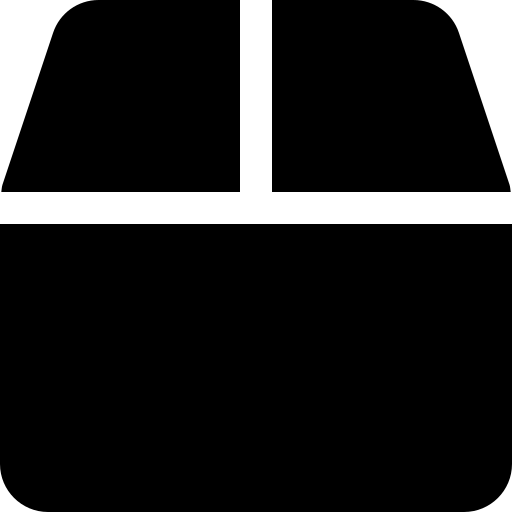
\includegraphics[width=2.5in]{box}%
%\label{fig_second_case}}
%\caption{Simulation results.}
%\label{fig_sim}
%\end{figure*}
%
% Note that often IEEE papers with subfigures do not employ subfigure
% captions (using the optional argument to \subfloat[]), but instead will
% reference/describe all of them (a), (b), etc., within the main caption.


% An example of a floating table. Note that, for IEEE style tables, the 
% \caption command should come BEFORE the table. Table text will default to
% \footnotesize as IEEE normally uses this smaller font for tables.
% The \label must come after \caption as always.
%
%\begin{table}[!t]
%% increase table row spacing, adjust to taste
%\renewcomma\cite{chaum-dc}\cite{chaum-dc}nd{\arraystretch}{1.3}
% if using array.sty, it might be a good idea to tweak the value of
% \extrarowheight as needed to properly center the text within the cells
%\caption{An Example of a Table}
%\label{table_example}
%\centering
%% Some packages, such as MDW tools, offer better commands for making tables
%% than the plain LaTeX2e tabular which is used here.
%\begin{tabular}{|c||c|}
%\hline
%One & Two\\
%\hline
%Three & Four\\
%\hline
%\end{tabular}
%\end{table}


% Note that IEEE does not put floats in the very first column - or typically
% anywhere on the first page for that matter. Also, in-text middle ("here")
% positioning is not used. Most IEEE journals use top floats exclusively.
% However, Computer Society journals sometimes do use bottom floats - bear
% this in mind when choosing appropriate optional arguments for the
% figure/table environments.
% Note that, LaTeX2e, unlike IEEE journals, places footnotes above bottom
% floats. This can be corrected via the \fnbelowfloat command of the
% stfloats package.

\section{Discussion}

\subsection{Comparison to Existing Systems}
The following section gives a short comparison to existing systems. It shows that the solution defined in this paper covers a different approach and what problems are solved. It is important to note that this is not a ranking. It just outlines the differences between the system and shows where our system is different compared to existing solutions.

\subsubsection{TOR}
%TOR has attracted considerable efforts from the scientific community in both attacking and defence. As an immediate result numerous attacks and counter measures exist within TOR. It was however never designed to withstand such a harsh definition for an adversary as we used it. TOR fails therefore in several aspects. Numerous attacks as outlined previously will succeed when assuming our adversary. 
%
TOR is criticised for several things. Firstly, it is easy attackable if encryption is not used in the transported protocol. It relies on the trust in a centralized directory infrastructure. It is susceptible if more than $\approx 30\%$ of the nodes are controlled by an adversary as shown in \cite{jansen2014sniper}. Furthermore, timing analysis on entry and exit nodes are particularly easy due to the fact that TOR is a low latency network\cite{torta05,esorics10-bandwidth}. Harvesting of nodes is possible (e.g. \url{https://torstatus.blutmagie.de}). Tor nodes are easily identifiable by traffic as shown in \cite{foci12-winter}. To avoid this detection TOR uses ``pluggable transports''. Unlike in MessageVortex, this is not used in general but only when specifically set up between two nodes.

MessageVortex tries to address these problems in multiple ways. First, there is no central infrastructure which defies the trust problem. There are no entry or exit nodes as all participating members are routers at the same time. Therefore, all problems related to entry and exit nodes do not exist. There is no dedicated transport protocol making the presence of vmessages hard to detect.

MessageVortex has several downsides compared to TOR. It is not suitable for real time communication due to its asynchronous operation. It is furthermore a closed system and only participating members may use it. %In contrast, TOR allows to tunnel almost any traffic through it to any destination. 

\subsubsection{$\mathcal{P}^5$}
%The Peer-to-Peer Personal Privacy Protocol is defined in \cite{sherwood2005p5}. It provides sender-, receiver- and sender-receiver anonymity. According to the project page of $\mathcal{P}^5$ there is only a simulator available for the protocol.
%
%The transport layer issue has been completely ignored. 
In-depth analysis of $\mathcal{P}^5$ is very limited, as there is no true protocol specification but only a rough outline available. This outline specifies the messaging and the crypto operations only. It claims to be peer to peer, which would result in some kind of NAT (Network Address Translation) circumvention technology. This technology usually relies, at least partially, on a central infrastructure (e.g. for hole punching). 

In contrast MessageVortex protocol is peer to peer but the transport layer is not. It misuses already existing infrastructure for transport. This makes it not susceptible to approaches against infrastructure unless our messages are identified and filtered. This may be corrected by applying different blending schemes for the transport layer. It furthermore removes the need for NAT hole punching and similar technologies.

\subsubsection{$I^2P$}
%The name $I^2P$ is derived from  ``Invisible Internet Project'' according to \href{https://geti2p.net/}{geti2p.net}. The system itself is comparable to TOR in its capabilities. Mayor differences are:
%\begin{itemize}
%	\item P2P based
%	\item Packet switched routing (TOR is ``circuit switched'')
%	\item Different forward and backward routes (called tunnels)
%	\item Works pseudonymously
%	\item Supports TCP and UDP
%\end{itemize}
%
$I^2P$ has not attracted as much attention as TOR so far. It is thus hard to judge its real qualities. 

Unlike TOR, anonymity is not fully granted. Instead a pseudonymity is used. 

In \cite{pets2011-i2p} an attack specific to $I^2P$ is presented. As $I^2P$s security model is chosen based on IP addresses, the authors propose to use several cloud providers in different B-Class networks. By selectively flooding peers, an adversary may extract statistical information. The paper proposes an attack based on the heuristic performance-based peer selection. The main criticism of the paper were that the peer selection may be influenced by an adversary enabling him to recover data on a statistical base.

MessageVortex does only allow a routing block builder to choose routes and amount of traffic. Due to the replay protection and the trust, we do not rely on any node, we show in \cite{messageVortex} that attacks on this level are not possible.

\subsubsection{Freenet}
%Freenet was originally designed to be a fully distributed data store\cite{freenet}. Documents are stored in an encrypted form. Downloaders must know a document descriptor called CHK containing the file hash, the key, and some background about the crypto being used. A file is stored more or less redundantly based on the number of accesses to a stored file. The main goal of Freenet is to decouple  authorship from a particular document. It furthermore provides a fault tolerant storage, which improves caching of a document if requested more often.
%
While Freenet is a pure distributed storage system it has many good features adapted by MessageVortex. Like in Freenet a MessageVortex node may deny to be the owner of a specific information unless the key for the respective ephemeral identity can be found on the system. As the key is only required for building routing blocks but not for message assembly and sending, this makes it a valuable feature comparable to the deniability of Freenet.

\section{Conclusion}
The MessageVortex protocol outlined in the previous sections does not solve all privacy issues which might arise. Furthermore, it is complicated to implement and involves a considerable amount of book keeping at runtime which is left to the sender of a message and the mixing nodes. 

On the positive side, we have a new protocol which addresses privacy in a holistic approach leaving very little attack surface. If handled with appropriate care by the sender and receiver, the protocol allows a sender-controlled, high degree amount of anonymity. Message paths are diagnosable, may be built redundant and do not build on the trust of any third party systems including all involved mixes except the sender's and receiver's one. Even closed group communication or broadcasting to multiple identities involving a specific subset of mixes is possible if desired by the sender.

In \cite{messageVortex} we show that the protocol is very secure. It is hard to block as messages may be redundant, hard to identify as messages are covered within message flows which may not be blocked without huge impact on existing systems. It is hard to apply censorship in a real world scenario as messages are extremely hard to detect. 

MessageVortex has some flaws which must be outlined. We always considered an algorithmic censorship. If human censorship is applied, we must assume that at least some of the messages are being identified as possible MessageVortex messages. If we assume a white-listing, human, censoring adversary (everything which is not identified by a human as compliant is censored) we must conclude that at least some messages will fail to be delivered. 

Some of the participating transport nodes may be identified and blocked. This may be compensated with redundancy in message transmission. 

Messages transported by MessageVortex generate huge amounts of decoy traffic. Unlike other systems which control decoy traffic on a ``per peer'' base, MessageVortex does not dynamically reduce decoy traffic as decoy traffic is not identifiable. This results in a huge traffic overhead.


% if have a single appendix:
%\appendix[Proof of the Zonklar Equations]
% or
%\appendix  % for no appendix heading
% do not use \section anymore after \appendix, only \section*
% is possibly needed

% use appendices with more than one appendix
% then use \section to start each appendix
% you must declare a \section before using any
% \subsection or using \label (\appendices by itself
% starts a section numbered zero.)
%

\newpage
\appendices

\section{Reed-Solomon Function\label{sec:reedSolomon}}
The origins of the Reed-Solomon code go back to \cite{reed1960polynomial}. The method described in this paper was however not applicable in all cases. The publications \cite{karnin1983secret} and \cite{Rabin:1989:EDI:62044.62050} describe a more practical solution whereas \cite{preparata1989holographic} brings up the similarity to the Reed-Solomon code with a $GF(2^\omega)$. 

Reed-Solomon is used for many applications today. One of the most well known application is a redundancy generator for RAID-6 like systems. It is able to generate multiple linearly independent equation systems to a given set of data $B_1\ldots B_{n-m}$ creating redundancy information $R_1\ldots R_m$. In a system with all blocks $\langle B_1\ldots B_{n-m}, R_1\ldots R_m \rangle$ any number $k$ where $0\le k\le m$ datablocks may be removed and the information contained in $\langle B_1\ldots B_{n-m}\rangle$ is still recoverable. 

Traditionally the data and redundancy information is striped into blocks and distributed together with the redundancy information over all $n$ storages. This is done to avoid data storages as bottleneck since a change to one data stripe  in a stripe set results always in a change of the redundancy data on the other $m$ redundancy storages. This would result in hot spots on redundancy information storages.

We use the Reed-Solomon function as redundancy generating function shown in Fig~\ref{fig:addRedundancy}. Unlike in storage technology we encrypt each redundancy block and all data stripes individually. By doing so we make it impossible to recover the contained information without knowledge of the keys. All blocks do then contain the same amount of data. Given we have enough blocks and the corresponding keys we may rebuild the message. 

At the same time the generating node is unable to tell what blocks belong to the true message path and what blocks are sent for decoy traffic only. 

As our resulting blocks are encrypted with a stream or block cypher, we need to introduce some padding. The padding is applied before doing RS calculation. In the case of a stream cypher we need to pad so that the number of bytes is dividable by the number of data blocks. In the case of block cyphers we need to pad so that all resulting data blocks have exactly a size dividable by the block size. We achieve two goals by applying the padding before spliting the blocks. First we reduce overhead by adding only one instead of $n$ paddings. Secondly, an unpadded block is much harder to brute force. Any resulting block to a key might be the right one as we no longer have padding to suggest that a decryption has been successful.

We defined to use Vandermonde matrices as outlined in \cite{pd:96:rs} and in \cite{pd:03:rs} for our redundancy calculations. For more information of the used GF-Fields and exact matrix building instructions see \cite{messageVortex}.

\section{Pseudo Random Number Generator\label{sec:prng}}
Our PRNG used for this work is an xorshift+ generator. It is based on the XSadd PRNG\cite{marsaglia2003xorshift} and passes the bigcrush PRNG test suite. It is a fast, xor based PRNG which has two internal 64 bit seed states $s_0$ respectively $s_1$ and is defined as follows:

\begin{eqnarray}
x & = & s_0\\
s_0 & = & s_1\\
x & = & x \oplus ( x \ll 23 )\\
s_1 & = & x \oplus s_1 \oplus ( x \gg 17 ) \oplus (s_1 \gg 26 )\\
nextNumber & = & s_1+s_0
\end{eqnarray}

We have chosen this comparably weak PRNG for practical reasons. It is fast, simple, and is based on operations easy to implement on hardware. As we do not need a cryptographically strong PRNG, it is the primary choice so far. 

As the protocol is heavily dependent on security we have introduced everywhere at least one alternate algorithm which may be used if one of the choices may become a problem. In order to have a second choice for the PRNG we define the Blum-Micali PRNG as described in \cite{blum1984generate}. This PRNG is a cryptographically secure PRNG and is defined as follows:

$p$ is prime and $g$ is a primitive root modulo $p$. $x_0$ reflects the seed state.

\begin{eqnarray}
x_{i+1}=g^{x_i}\mod p
\end{eqnarray}


\section{Adversary Model\label{sec:adversary}}
We assume as an adversary a state-sponsored actor who has unlimited monitoring possibilities on the network layer within a limited geographic region (e.g. country). We furthermore assume available funding and capabilities to efficiently run a considerable number of nodes (not exceeding the number of $70\%$) within the network and harvest and combine all operations and content processed by these nodes.

This means he is at least capable of analysing traffic by algorithms and may disrupt any unwanted traffic.

The adversary is capable of generating any traffic anywhere within the message flow.

This is an adversary model which goes far beyond any model we have encountered in any other scientific approach.

Assumptions in this part are mostly derived from \cite{foci12-winter} and extrapolated. In this paper researchers describe GFC (Great Firewall of China) as a profiling firewall fingerprinting traffic and blocking specific socket addresses when positively identified as TOR nodes. 

\subsection{Detection\label{sec:detCons}}
Any adversary may use detection schemes to detect traffic. This may be used to apply censorship later. He is capable of analysing up to $1\%$ of the total transfer volume on an in-depth algorithmic base and $50\%$  based on simple context-less rules. 

\subsection{Censorship}
We assume that an adversary is accepting considerable economic damage but not the downfall of its own economy as a whole. An active adversary may apply algorithmic censorship based on the detection constraint (\ref{sec:detCons}) on a large scale.

\subsection{Information Retrieval}
We assume an adversary to be interested in all sorts of information available around messages. We consider the triple ``sender'', ``receiver'', and ``content'' as the most valuable set of information for an adversary. Other important informations are:

\begin{itemize}
	\item frequency of message interchange
	\item message size
\end{itemize}

For the system we consider the following information as interesting for an adversary (descending order):
\begin{itemize}
	\item Routing nodes
	\item Transporting nodes
	\item Routing operations
	\item Routing (ephemeral) identities
	\item Routing volumes
\end{itemize}


% you can choose not to have a title for an appendix
% if you want by leaving the argument blank

% use section* for acknowledgement
\ifCLASSOPTIONcompsoc
  % The Computer Society usually uses the plural form
  \section*{Acknowledgments}
\else
  % regular IEEE prefers the singular form
  \section*{Acknowledgment}
\fi
The authors would like to thank their families for being so patient with them, and all people which took the time to review the paper, criticised it, and their questions outlining the papers weaknesses.

% Can use something like this to put references on a page
% by themselves when using endfloat and the captionsoff option.
\ifCLASSOPTIONcaptionsoff
  \newpage
\fi



% trigger a \newpage just before the given reference
% number - used to balance the columns on the last page
% adjust value as needed - may need to be readjusted if
% the document is modified later
%\IEEEtriggeratref{8}
% The "triggered" command can be changed if desired:
%\IEEEtriggercmd{\enlargethispage{-5in}}

% references section

% can use a bibliography generated by BibTeX as a .bbl file
% BibTeX documentation can be easily obtained at:
% http://www.ctan.org/tex-archive/biblio/bibtex/contrib/doc/
% The IEEEtran BibTeX style support page is at:
% http://www.michaelshell.org/tex/ieeetran/bibtex/
\bibliographystyle{IEEEtran}
% argument is your BibTeX string definitions and bibliography database(s)
\bibliography{IEEEabrv,../inc/bib/unclassified/Anonbib/anonbib,../messagevortex}
%\bibliography{IEEEabrv,../bib/paper}
%
% <OR> manually copy in the resultant .bbl file
% set second argument of \begin to the number of references
% (used to reserve space for the reference number labels box)
%\begin{thebibliography}{1}
%
%\bibitem{IEEEhowto:kopka}
%H.~Kopka and P.~W. Daly, \emph{A Guide to {\LaTeX}}, 3rd~ed.\hskip 1em plus
%  0.5em minus 0.4em\relax Harlow, England: Addison-Wesley, 1999.
%
%\end{thebibliography}

% biography section
% 
% If you have an EPS/PDF photo (graphicx package needed) extra braces are
% needed around the contents of the optional argument to biography to prevent
% the LaTeX parser from getting confused when it sees the complicated
% \includegraphics command within an optional argument. (You could create
% your own custom macro containing the \includegraphics command to make things
% simpler here.)
%\begin{IEEEbiography}[{\includegraphics[width=1in,height=1.25in,clip,keepaspectratio]{mshell}}]{Michael Shell}
% or if you just want to reserve a space for a photo:
\ifCLASSOPTIONpeerreview
\else
\vfill
\begin{IEEEbiography}[{\includegraphics[width=1in,height=1.25in,clip,keepaspectratio]{../inc/biography/passphoto}}]{Martin Gwerder}
% !TeX spellcheck = en_GB

Martin Gwerder was born 20. July 1972 in Glarus, Switzerland. He is currently a doctoral Student at the University of Basel. After having concluded his studies at the polytechnic at Brugg in 1997, he did a postgraduate study as a master of business and engineering. Following that, he changed to the university track doing an MSc in Informatics at FernUniversit\"at in Hagen. While doing this he constantly broadened his horizon by working for industry, banking and government as  engineer and architect in security related positions. He currently holds a lecturer position for cloud and security at the University of Applied Sciences Northwestern Switzerland. His main expertise lays in the field of networking related problems dealing with data protection, distribution, confidentiality and anonymity.
\end{IEEEbiography}
\fi

% if you will not have a photo at all:
%\begin{IEEEbiographynophoto}{John Doe}
%Biography text here.
%\end{IEEEbiographynophoto}

% insert where needed to balance the two columns on the last page with
% biographies
%\newpage

%\begin{IEEEbiographynophoto}{Jane Doe}
%Biography text here.
%\end{IEEEbiographynophoto}

% You can push biographies down or up by placing
% a \vfill before or after them. The appropriate
% use of \vfill depends on what kind of text is
% on the last page and whether or not the columns
% are being equalized.

%\vfill

% Can be used to pull up biographies so that the bottom of the last one
% is flush with the other column.
%\enlargethispage{-5in}



% that's all folks
\end{document}


